
\documentclass[11pt]{article}
\usepackage[margin=1in]{geometry}
\usepackage{amsmath,amssymb,amsfonts,bm}
\usepackage{booktabs}
\usepackage{graphicx}
\usepackage{hyperref}
\usepackage{enumitem}
\usepackage{xcolor}
\usepackage{float}
\hypersetup{colorlinks=true,linkcolor=blue,urlcolor=blue,citecolor=blue}
\title{Phase 6 Technical Specification\\Consensus Sheaf Discovery and Reliability}
\author{Sheaf-Theoretic Multi-Omics Brain Tumor Project}
\date{May 2026}
\begin{document}
\maketitle
\tableofcontents
\newpage

\section{Purpose}
Phases 1--5 constructed patient-level sheaf inconsistency energies, learned restriction maps, subtype-specific sheaf geometries, and optimal-transport stability. Phase 6 adds the discovery layer. Its objective is to identify sheaf residual features that are not only predictive, but also stable, statistically associated with biological labels, robust to permutation, and interpretable as regulatory inconsistency signatures.

The central Phase 6 object is the \emph{Consensus Sheaf Discovery Score} (CSDS), which ranks candidate sheaf features by combining sparse-model stability, marginal biological effect, false-discovery control, and transport stability.

\section{Candidate Feature Family}
For each patient $p$, let
\[
\mathbf{s}(p)=\left[\operatorname{SRIS}(p), E_{D\to R}(p), E_{D\to C}(p), E_{R\to C}(p), \ldots \right]
\]
collect Phase 1 residuals, Phase 4 counterfactual sheaf energies, and Phase 5 transport-to-reference distances. A candidate sheaf feature is one coordinate
\[
\phi_j(p)=s_j(p).
\]
These features are evaluated under strict leakage-control protocols, including no-IDH/no-grade/no-cluster variants when the endpoint would otherwise be partially encoded by the inputs.

\section{Sparse Stability Selection}
For task $t$ with labels $y_p$, repeated stratified folds are constructed. On each training fold, a sparse logistic model is fit on sheaf candidates:
\[
\widehat{\beta}^{(b)}
=\arg\min_{\beta}
\left\{\mathcal{L}_t(\beta;X^{(b)},y^{(b)})+\lambda\|\beta\|_1\right\}.
\]
The selection frequency of feature $j$ is
\[
\pi_j=\frac{1}{B}\sum_{b=1}^B \mathbf{1}\{\widehat{\beta}^{(b)}_j\ne 0\}.
\]
This prevents the paper from relying only on one fitted model or one lucky train-test split.

\section{Association and Permutation Testing}
For each feature $\phi_j$, Phase 6 computes a task-specific association statistic. For binary tasks, it uses a rank-based two-group statistic; for multiclass tasks, it uses a Kruskal--Wallis statistic. Let the observed statistic be $T_j$. Under label permutations $\sigma_1,\ldots,\sigma_M$, the empirical p-value is
\[
\widehat{p}_j
=\frac{1+\sum_{m=1}^{M}\mathbf{1}\{T_j(\sigma_m y)\ge T_j(y)\}}{M+1}.
\]
The empirical p-values are adjusted by Benjamini--Hochberg FDR to obtain $q_j$.

\section{Transport-Calibrated Stability Weight}
Phase 5 estimated edge-wise transport stability between biological groups. Phase 6 maps each feature to an edge family and assigns a transport stability weight
\[
\tau_j\in[0,1].
\]
For example, a feature involving $D\to R$ receives the average Phase 5 $D\to R$ stability, while total-energy features receive the SRIS-level stability. This gives priority to features that remain coherent under cross-group transport.

\section{Consensus Sheaf Discovery Score}
Let $a_j$ be the normalized marginal effect size of feature $j$, $\pi_j$ its stability-selection frequency, $q_j$ its FDR value, and $\tau_j$ its transport stability. Phase 6 defines
\[
\boxed{
\operatorname{CSDS}_j
=\pi_j\,a_j\,(1-q_j)\,\tau_j.
}
\]
A high-CSDS feature is repeatedly selected, associated with the endpoint, FDR-supported, and transport-stable.

\section{Patient-Level Sheaf Discovery Index}
For each task, the top $K$ CSDS-ranked features are combined into a patient-level Sheaf Discovery Index:
\[
\operatorname{SDI}(p)=
\sum_{j\in\mathcal{T}_K} w_j\,z(\phi_j(p)),
\]
where $z(\cdot)$ denotes cohort standardization and
\[
w_j\propto \operatorname{sign}(\bar{\beta}_j)\operatorname{CSDS}_j.
\]
This creates a compact one-dimensional summary of the most reliable sheaf-discovery signal for a task.

\section{Internal Results}
Phase 6 produced a discovery table, patient-level SDI table, prediction metrics, cross-task consensus table, and figures. The most important tables are summarized below.

\subsection{Best Accuracy Deltas}
\begin{center}
\input{phase6_best_delta_table.tex}
\end{center}

\subsection{Top Consensus Sheaf Discoveries}
\begin{center}
\resizebox{\textwidth}{!}{\input{phase6_top_feature_table.tex}}
\end{center}

\section{Figures}
\begin{figure}[H]
\centering
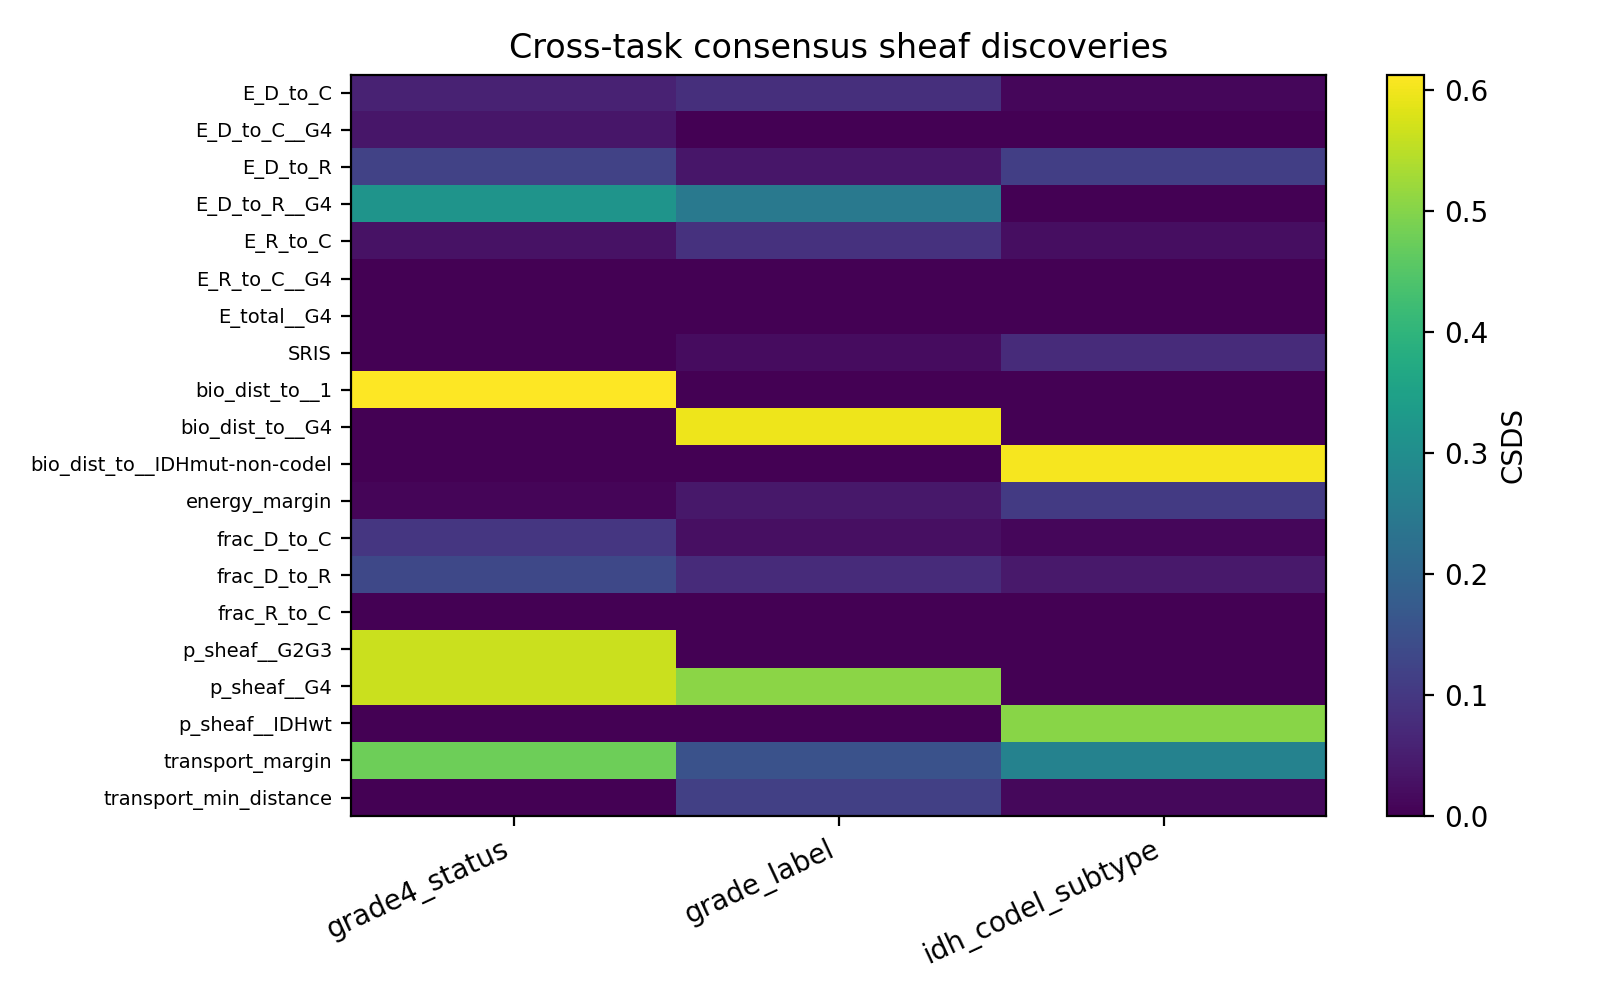
\includegraphics[width=.9\textwidth]{../figures/phase6_cross_task_CSDS_heatmap.png}
\caption{Cross-task consensus sheaf discovery heatmap.}
\end{figure}

\begin{figure}[H]
\centering
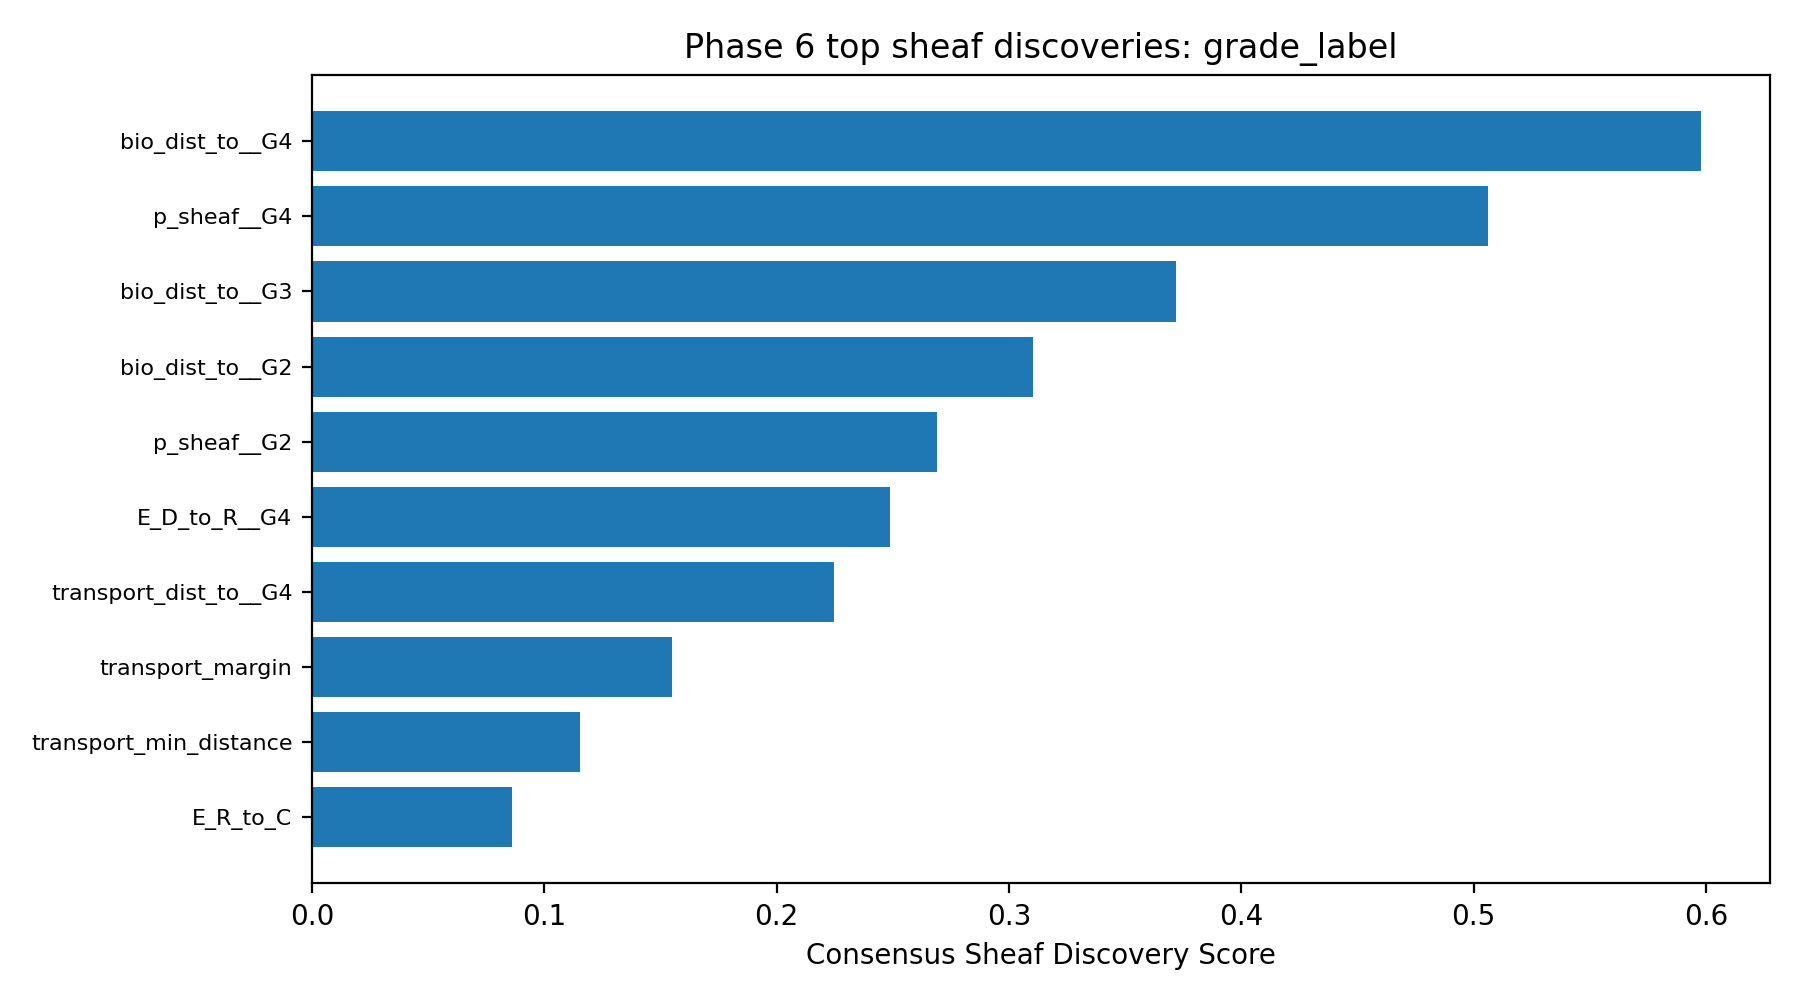
\includegraphics[width=.9\textwidth]{../figures/phase6_top_CSDS_grade_label.png}
\caption{Top Phase 6 CSDS features for strict grade classification.}
\end{figure}

\section{Interpretation}
Phase 6 creates a new discovery layer: the model now produces uncertainty-aware, transport-calibrated sheaf residual biomarkers rather than only classification scores. This is technically distinct from ordinary multi-omics feature fusion because each candidate feature is derived from a sheaf residual, group-specific sheaf energy, or transport-calibrated sheaf distance.

The correct current interpretation is that Phase 6 improves internal biological-discovery rigor and identifies candidate residual signatures. These signatures remain internal until tested on an external cohort such as CGGA.

\section{Deliverables}
\begin{itemize}[leftmargin=*]
\item \texttt{phase6\_consensus\_feature\_discovery.csv}: feature-level CSDS table.
\item \texttt{phase6\_patient\_sheaf\_discovery\_index.csv}: patient-level SDI scores.
\item \texttt{phase6\_prediction\_metrics.csv}: cross-validated prediction metrics.
\item \texttt{phase6\_metric\_deltas.csv}: baseline vs Phase 6 improvements.
\item \texttt{phase6\_cross\_task\_consensus.csv}: recurrent discoveries across tasks.
\item Figures for CSDS rankings, SDI distributions, and cross-task consensus.
\end{itemize}

\end{document}
